\chapter{Experiment Environments}

\section{FutureGrid}

\section{WorkflowSim}

WorkflowSim is an open source workflow simulator that extends CloudSim \cite{Calheiros2011} by providing a workflow level support of simulation. It models workflows with a DAG model with support an elaborate model of node failures, a model of delays occurring in the various levels of the WMS stack \cite{Chen2011}, the implementations of several most popular dynamic and static workflow schedulers (e.g., HEFT, Min-Min) and task clustering algorithms (e.g., runtime-based algorithms, data-oriented algorithms and fault tolerant clustering algorithms). Parameters are imported from Models and Trace Analysis. Workflow DAG model (represented as a DAX (DAG in XML) file is imported from WorkflowGenerator.  

In this section, we introduce our workflow simulator called WorkflowSim that utilizes the o-DAG model to simulate large scale workflows. We verify its effectiveness through a series of experiments. The evaluation of the performance of workflow optimization techniques in real infrastructures is complex and time consuming. As a result, simulation-based studies have become a widely accepted way to evaluate workflow systems. For example, scheduling algorithms, such as HEFT \cite{Topcuoglu2002}, MaxMin \cite{Braun2001}, MinMin \cite{Blythe2005}, etc., have used simulators to evaluate their effectiveness. A simulation-based approach reduces the complexity of the experimental setup and saves much effort in workflow execution by enabling the testing of their applications in a repeatable and controlled environment. 


\begin{figure}[h!]
	\centering
    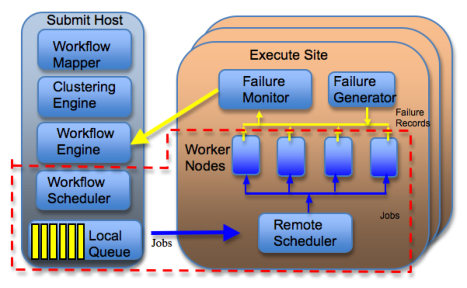
\includegraphics[width=0.7\textwidth]{figures/model/wfs_overview.pdf}
    \caption{WorkflowSim Overview. The area surrounded by red lines is supported by CloudSim}
    \label{fig:model_wfs_overview}
\end{figure}

However, an accurate simulation framework for scientific workflows is required to generate reasonable results, particularly considering that the overall system overhead \cite{Overhead2011} plays a significant role in the workflow’s runtime. 
%In heterogeneous distributed systems, workflows may experience different types of overheads, which are defined as the time of performing miscellaneous work other than executing users’ computational activities.  Since the causes of overheads differ, the overheads have diverse distributions and behaviors. For example, the time to run a post-script that checks the return status of a computation is usually a constant. However, queue delays incurred while tasks are waiting in a batch scheduling systems can vary widely. 
By classifying these workflow overheads in different layers and system components, our simulator can offer a more accurate result than simulators that do not include overheads in their system models.

What’s more, many researchers \cite{Zhang2004, Tang1990, Schroeder2006, Sahoo2004, Oppenheimer2002, Mcconnel} have emphasized the importance of fault tolerant design and concluded that the failure rates in modern distributed systems should not be neglected. A simulation with support for randomization and layered failures is supported in WorkflowSim to promote such studies. 

Finally, progress in workflow research also requires a general-purpose framework that can support widely accepted features of workflows and optimization techniques. Existing simulators such as CloudSim/GridSim \cite{Calheiros2011} fail to provide fine granularity simulations of workflows. For example, they lack the support of task clustering, which is a popular technique that merges small tasks into a large job to reduce task execution overheads. The simulation of task clustering requires two layers of execution model, on both task and job levels. It also requires a workflow-clustering engine that launches algorithms and heuristics to cluster tasks. Other techniques such as workflow partitioning and task retry are also ignored in these simulators. These features have been implemented in WorkflowSim. 

%To the best of our knowledge, none of the current distributed system simulators support these rich-features and techniques. In this section, we introduce our early work on simulating scientific workflows satisfying these requirements. We evaluate the performance of WorkflowSim with an example of task clustering. We further show that WorkflowSim is promising in providing an evaluation platform for research areas such as fault tolerant clustering and overhead robustness studies. 

\subsection{Components and Functionalities}

\begin{figure}[!htb]
	\centering
	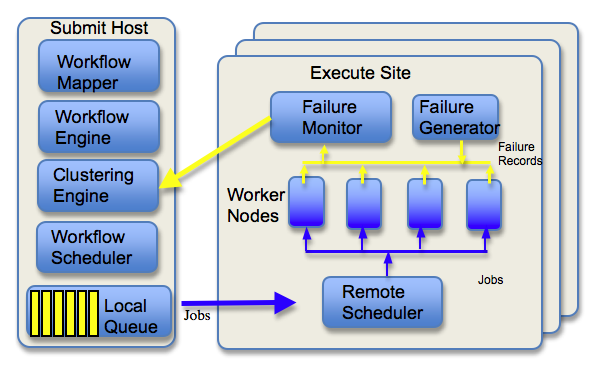
\includegraphics[width=1.0\linewidth]{figures/workflowsim/wfs_overview.png}
	\caption{Overview of WorkflowSim.}
	\label{fig:wfs}
\end{figure}

Deelman et. al. \cite{Deelman2009} have provided a survey of popular workflow systems for scientific applications and have classified their components into four categories: composition, mapping, execution, and provenance. Based on this survey, we identified the mandatory functionalities/components and designed the layers in our WorkflowSim. In our design as shown in Figure~\ref{fig:wfs}, we add multiple layers on top of the existing task scheduling layer of CloudSim, which include Workflow Mapper, Workflow Engine, Clustering Engine, Workflow Scheduler, Failure Generator and Failure Monitor etc. 

\subsubsection{Workflow Mapper} is used to import DAG files formatted in XML (called DAX in WorkflowSim) and other metadata information such as file size from Workflow Generator. Workflow Mapper creates a list of tasks and assigns these tasks to an execution site. A task is a program/activity that a user would like to execute. 
\subsubsection{Workflow Engine} manages tasks based on their dependencies between tasks to assure that a task may only be released when all of its parent tasks have completed successfully. The Workflow Engine will only release free tasks to Clustering Engine. 
\subsubsection{Clustering engine} merges tasks into jobs such that the scheduling overhead is reduced. A job is an atomic unit seen by the execution system, which contains multiple tasks to be executed in sequence or in parallel if applicable. Different to the clustering engine in Pegasus WMS, Clustering Engine in WorkflowSim also perform task reclustering in a faulty environment with transient failures. If there are failed tasks returned from Workflow Scheduler, they are merged again into a new job.  
\subsubsection{Workflow Scheduler} is used to match jobs to a worker node based on the criteria selected by users. WorkflowSim relies on CloudSim to provide an accurate and reliable job-level execution model, such as time-shared model and space-shared model. However, WorkflowSim has introduced different layers of overheads and failures based on our prior work \cite{Chen2011}, which improves the accuracy of simulation. 
\subsubsection{Failure Generator} is introduced to inject task/job failures at each execution site during the simulation. After the execution of each job, Failure Generator randomly generates task/job failures based on the distribution and average failure rate that a user has specified. 
\subsubsection{Failure Monitor} collects failure records (e.g., resource id, job id, task id) to return these records to Clustering Engine to adjust the scheduling strategies dynamically. In a failure-prone environment, there are several options to improve workflow performance. First, one can simply retry the entire job or only the failed part of this job when its computation is not successful.  This functionality is added to the Workflow Scheduler, which checks the status of this job and takes action based on the strategies that a user selects. 


WorkflowSim extracts the common features exposed by various workflow systems and supports widely used workflow features and optimization techniques. Below we list the main functionalities supported by WorkflowSim. Note that WorkflowSim is an open source community and more functionalities are added at the same time. 

\subsubsection{Overhead Modeling} Based on our prior studies on workflow overheads \cite{Chen2011}, we add layered overhead to the workflow simulation. We have classified workflow overheads into five categories as follows. Workflow Engine Delay measures the time between when the last parent job of a job completes and the time when the job gets submitted to the local queue. Queue Delay is defined as the time between the submission of a job by the workflow engine to the local queue and the time the local scheduler sees the job running. Data Transfer Delay happens when data is transferred between nodes. Clustering Delay measures the difference between the sum of the actual task runtime and the job runtime seen by the Workflow Scheduler. 
\subsubsection{Failure Modeling} WorkflowSim supports two types failures. A task failure which means a task fails while other tasks in the same job may not fail. A job failure means a job fails while all of its tasks fail. The reason why we have this classification of transient failures is that they usually have different causes. Task failure is usually generated by an error during the execution while a job failure happens during the preparation of a job.   Users can specify the distribution (Weibull, Uniform, Normal and Gamma) of the failure rates. 
\subsubsection{Shared and Distributed File Systems} 
Modern file systems are usually classified into two types. The first one is a central file system in which the data storage is shared among all the worker nodes in a data-center. The communication cost is thereby included in the execution time of a task and scheduling algorithms do not necessary consider the data transfer delay between tasks. The second is a distributed file system in which the data storage is constructed with multiple separate local data storages. The communication cost should not be ignored and data-aware scheduling algorithms can apply to this environment to optimize the data locality and the overall makespan. In either way, WorkflowSim uses a Replica Catalog to keep track of the files including their replications. 
\subsubsection{Dynamic Scheduling Algorithm} While CloudSim has already supported static scheduling algorithms, we added the support of dynamic workflow algorithms in WorkflowSim. For static algorithms, jobs are assigned to a worker node at the workflow planning stage. When a job reaches the remote scheduler, it will just wait until the assigned worker node is free. For dynamic algorithms, jobs are matched to a worker node in the remote scheduler whenever a worker node becomes idle. This classification proposes new options for researchers to evaluate the dynamic performance of their algorithms. 
\subsubsection{Task Clustering} Compared to CloudSim and other workflow simulators, WorkflowSim provides support of task clustering that merges tasks into a clustered job. Users can specify different criteria to optimize the overall performance. For example, in a fault environment, a long job would end up with running forever even though the overheads are reduced. 
\subsubsection{Energy aware}

As Fig~\ref{fig:model_wfs_overview} shows, there are multiple layers of components involved in preparing and executing a workflow. Among them, Workflow Mapper, Workflow Engine, Workflow Scheduler and Job Execution have been introduced in last section. Below we introduce three components that have not been introduced. 
\begin{enumerate}

\item Clustering Engine

The Clustering Engine merges tasks into jobs so as to reduce the scheduling overheads. 

%\item Workflow Engine 

%The Workflow Engine manages jobs based on their dependencies to assure that a job may only be released when all of its parent jobs have completed successfully. The Workflow Engine will only release free jobs to the Scheduler. In the real execution we studied, we use DAGMan \cite{DAGMan} as the Workflow Engine. 
  
%\item Workflow Scheduler and Job Execution

%The Workflow Scheduler is used to match jobs to worker nodes based on the criteria selected by users (MaxMin \cite{Braun2001}, MinMin \cite{Blythe2005} , and many other heuristics). While CloudSim has already supported static scheduling algorithms, we added the support of dynamic workflow algorithms. For static algorithms, jobs are assigned to a worker node at the workflow planning stage. When the job reaches the remote scheduler, it will just wait until the assigned worker node is free. For dynamic algorithms, jobs are matched to a worker node in the remote scheduler whenever a worker node becomes idle. WorkflowSim relies on CloudSim to provide an accurate and reliable job-level execution model, such as time-shared model and space-shared model. However, WorkflowSim has introduced different layers of overheads and failures, which improves the accuracy of simulation. 

%\begin{figure}[h!]
%	\centering
 %   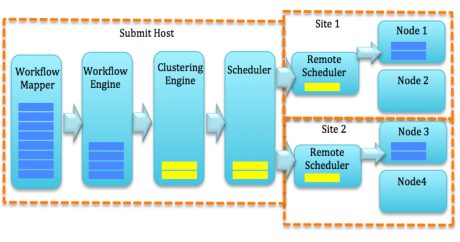
\includegraphics[width=0.7\textwidth]{figures/model/wfs_interaction.pdf}
  %  \caption{Interaction between components}
   % \label{fig:model_wfs_interaction}
%\end{figure}


%To associate and coordinate these layers, we adopted an event-based approach where each component maintains a message queue. Fig~\ref{fig:model_wfs_interaction} shows a simple configuration with two execution sites, of which each has two nodes. Each component maintains its own message queue and iteratively checks whether it can process one message. For example, at each iteration, the Clustering Engine checks whether it has received new tasks from the Workflow Engine and whether it should release new jobs to the Scheduler. When none of these components have any more messages in queue, the simulation is completed. 

%Based on our prior studies on workflow overheads, we add layered overhead to the workflow simulation. We have classified workflow overheads into five categories as follows. 
%\begin{enumerate}

%\item Workflow Engine Delay measures the time between when the last parent job of a job completes and the time when the job gets submitted to the local queue. In case of retries the value of the last retry is used for the calculation. Since we use a DAG model to represent workflows, the completion time of the last parent job means this job is released to the ready queue and is waiting for resources to be assigned to it. The workflow engine delay reflects the efficiency of a workflow engine (in our case DAGMan). 

%\item Queue Delay is defined as the time between the submission of a job by the workflow engine to the local queue and the time the local scheduler sees the job running (potentially on remote resources). This overhead reflects the efficiency of the workflow scheduler (e.g., Condor \cite{Frey2002}) to execute a job and the availability of resources for the execution of the job. In case of retries the value is the cumulative of all the retries.  
%\item Postscript Delay and Prescript Delay is the time taken to execute a lightweight script under some execution systems before and after the execution of a job. Prescripts are usually used to create directories for job execution. Postscripts examine the exit code of a job after the computational part of the job is done.
%\item Data Transfer Delay happens when data is transferred between nodes. It includes three different types of processes: staging data in, cleaning up, and staging data out. Stage-in jobs transfer input files from source sites to execution sites before the computation starts. Cleanup jobs delete intermediate data that is no longer needed by the remainder of the workflow. Stage-out jobs transfer workflow output data to archiving sites for storage and analysis.
%\item Clustering Delay measures the difference between the sum of the actual task runtime and the job runtime seen by the Workflow Scheduler. The cause of Clustering Delay is usually the use a job wrapper used to execute a clustered job. The wrapper takes some time to extract the list of tasks and to launch them. 
%\end{enumerate}                        

%Failures can occur at different times during the workflow execution. Consistent with the definition of tasks and job, we divide transient failures into two categories: task failure and job failure. If the transient failure affects the computation of a task (task failure), other tasks within the job do not necessarily fail. If the transient failure affects the clustered job (job failure), all of its tasks fail. We have added two components in response to the simulation of failures:
\item Failure Generator component is introduced to inject task/job failures at each execution site. After the execution of each job, Failure Generator randomly generates task/job failures based on the distribution and average failure rate that a user has specified. 
\item Failure Monitor collects failure records (e.g., resource id, job id, task id) and returns them to the workflow management system so that it can adjust the scheduling strategies dynamically. 
\end{enumerate}
We also modified other components to support fault tolerant optimization. In a failure-prone environment, there are several options to improve workflow performance. First, one can simply retry the entire job or only the failed part of this job when its computation is not successful. This functionality is added to the Workflow Scheduler, which checks the status of a job and takes action based on the strategies that a user selects. Furthermore, Reclustering is a technique that we have proposed \cite{Chen2012} that aims to adjust the task clustering strategy based on the detected failure rate. This functionality is added to the Workflow Engine. 

\subsection{Results and Validation}
We use task clustering as an example to illustrate the necessity of introducing overheads into workflow simulation. The goal was to compare the simulated overall runtime of workflows in case the information of job runtime and system overheads are known and extracted from prior traces. 
In this example, we collected real traces generated by the Pegasus Workflow Management System while executing workflows on FutureGrid \cite{FutureGrid}. We built an execution site with 20 worker nodes and we executed the Montage workflow five times in every single configuration of $k$, which is the maximum number of clustered jobs in a horizontal level. These five traces of workflow execution with the same $k$ is a training set or a validation set. 
%Partly illustrated by Figure 5, the results are stable enough to be used as a training set. 
We ran the Montage workflow with a size of 8-degree squares of sky. The workflow has 10,422 tasks and 57GB of overall data. We tried different k from 20 to 100, leaving us 5 groups of data sets with each group having 5 workflow traces. 
First of all, we adopt a simple approach that selects a training set to train WorkflowSim and then use the same training set as validation set to compare the predicted overall runtime and the real overall runtime in the traces. We define accuracy in this section as the ratio between the predicted overall runtime and the real overall runtime:
\begin{equation} \label{eq:model_wfs_accuracy}
Accuracy=\frac{Predicted~Overall~Runtime}{Real~Overall~Runtime}
\end{equation}
 \begin{figure}[h!]
	\centering
    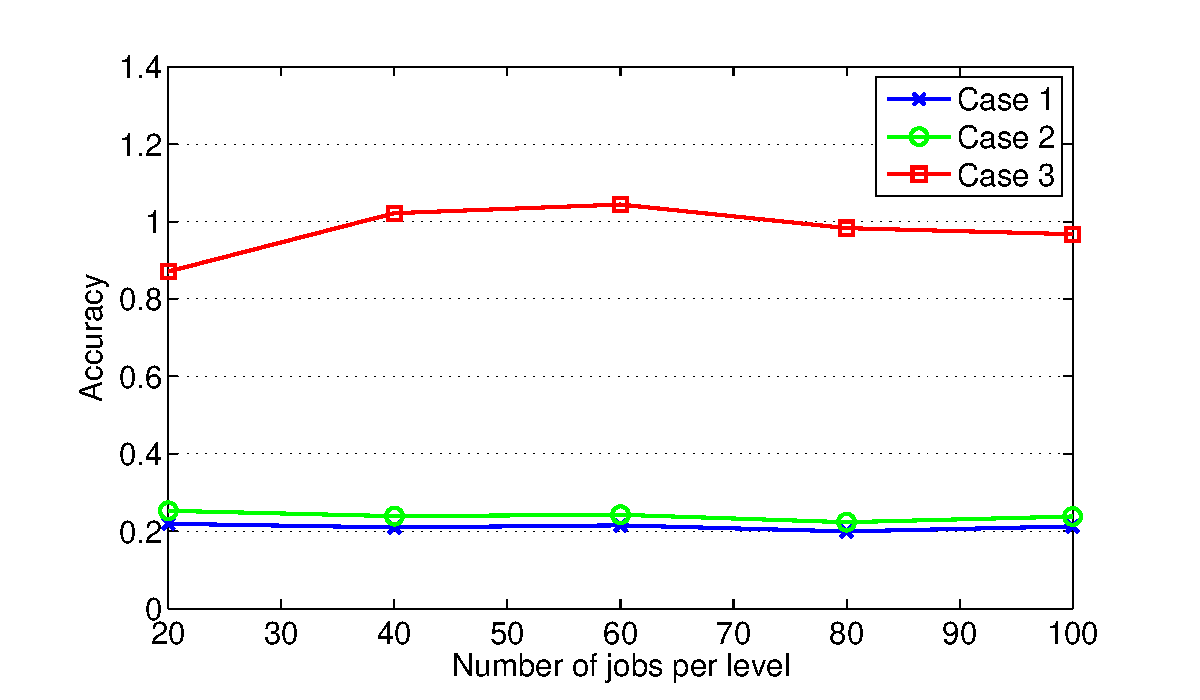
\includegraphics[width=0.9\textwidth]{figures/model/wfs_levels.eps}
    \caption{Performance of WorkflowSim with different support levels}
    \label{fig:model_wfs_levels}
\end{figure} 
 
Performance of WorkflowSim with different support levels. 
To train WorkflowSim, from the traces of workflow execution (training sets), we extracted information about job runtime and overheads, such as average/distribution and, for example, whether it has a cyclic increase. We then added these parameters into the generation of system overheads and simulated them as close as possible to the real cases. Here, we do not discuss the randomization or distribution of job runtime since we rely on CloudSim to provide a convincing model of job execution.

To present an explicit comparison, we simulated the cases using WorkflowSim that has no consideration of workflow dependencies or overheads (Case 1), WorkflowSim with Workflow Engine that has considered the influence of dependencies but ignored overheads (Case 2), and WorkflowSim, that has covered both aspects (Case 3). Intuitively speaking, we expect that the order of the accuracy of them should be Case 3 $>$ Case 2 $>$ Case 1. 

% \begin{figure}[h!]
%	\centering
%    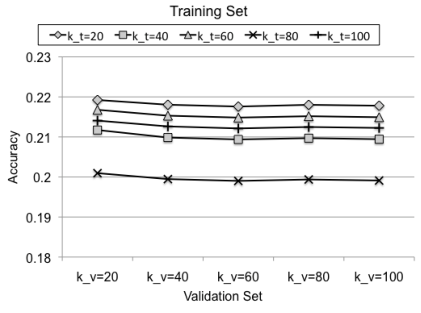
\includegraphics[width=0.6\textwidth]{figures/model/wfs_case1.pdf}
%    \caption{Performance of WorkflowSim of Case 1 (No workflow engine, or overhead support)}
 %   \label{fig:model_wfs_case1}
%\end{figure} 
 
%\begin{figure}[h!]
%	\centering
 %   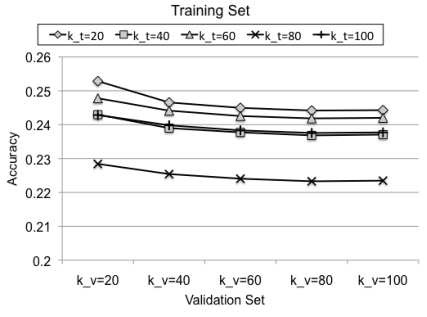
\includegraphics[width=0.6\textwidth]{figures/model/wfs_case2.pdf}
  %  \caption{Performance of WorkflowSim of Case 2 (No overhead support)}
    %\label{fig:model_wfs_case2}
%\end{figure} 

Fig~\ref{fig:model_wfs_levels} shows the performance of WorkflowSim with different support levels is consistent to our expectation. The accuracy of Case 3 is quite close to but not equal to 1.0 in most points. The reason is that to simulate workflows, WorkflowSim has to simplify models with a few parameters, such as the average value and the distribution type. It is not efficient to recur every overhead as is present in the real traces. It is also impossible to do since the traces within the same training set may have much variance. Fig~\ref{fig:model_wfs_levels} also shows that the accuracy of both Case 1 and Case 2 are much lower than Case 3. The reason why Case 1 does not give an exact result is that it ignores both dependencies and multiple layers of overheads. By ignoring data dependencies, it releases tasks that are not supposed to run since their parents have not completed (a real workflow system should never do that) and thereby reducing the overall runtime. At the same time, it executes jobs/tasks irrespective of the actual overheads, which further reduces the simulated overall runtime. In Case 2, with the help of Workflow Engine, WorkflowSim is able to control the release of tasks and thereby the simulated overall runtime is closer to the real traces. However, since it has ignored most overheads, jobs are completed and returned earlier than that in real traces. The low accuracy of Case 1 and Case 2 confirms the necessity of introducing overhead design into our simulator. 

%To further evaluate our task/job model and the performance of WorkflowSim, we adopted a cross-validation approach in which we picked up one group of data set (e.g., $k_t=20$) as input traces/training sets and simulated all the validation sets with $k_v=20$ to 100. To make it clear, we use $k_t$ to indicate the $k$ for a training set and $k_v$ for a validation set. Then we compare the accuracy in Fig~\ref{fig:model_wfs_case1}, Fig~\ref{fig:model_wfs_case2} and Fig~\ref{fig:model_wfs_case3} respectively. 
 
%\begin{figure}[h!]
%	\centering
%    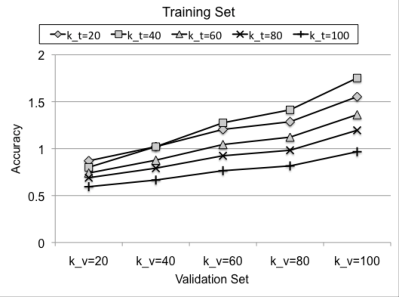
\includegraphics[width=0.6\textwidth]{figures/model/wfs_case3.pdf}
%   \caption{Performance of WorkflowSim of Case 3 (all features are enabled).}
%  \label{fig:model_wfs_case3}
%\end{figure} 

%Fig~\ref{fig:model_wfs_case1} and Fig~\ref{fig:model_wfs_case2} show similar conclusion as in Fig~\ref{fig:model_wfs_levels} and the accuracy of Case 2 and Case 1 are not sensitive to the task clustering. The reason is that Case 1 has no support of data dependencies, where jobs are all submitted at the beginning of workflow execution.  Case 2 has no support of system overhead and thereby task clustering does not improve the overall runtime much. Fig~\ref{fig:model_wfs_case3} shows the simulated results of WorkflowSim, which has considered both layered overhead and data dependencies. Although the accuracy is closer to 1.0, it still does not guarantee a 100\% accuracy in some cases. Particularly when we use a training set with a smaller k (e.g., $k_t=20$) to simulate the case with larger k (e.g., $k_v=100$), the accuracy suffers (accuracy=1.8). The reason is that the average Clustering Delay in the case of $k=20$ is much larger than that of other cases (as shown in Fig~\ref{fig:model_wfs_case2}), and thereby it is still larger than the predicted one using an inverse proportion function. Using such a large Clustering Delay to simulate the case with many clustered jobs ($k_v$ is large) would extend the predicted overall runtime of workflow. Our model has simplified and classified the distribution of overheads based on the horizontal level of tasks but we still need to further study the overhead distribution in accordance to different clustering strategies. However, a complex model may limit its general usage.  

%\subsection{Applications}

%With the features introduced in last section, we are able to carry out research studies such as evaluation of overhead robustness of DAG scheduling heuristics

%\begin{figure}[h!]
%	\centering
%    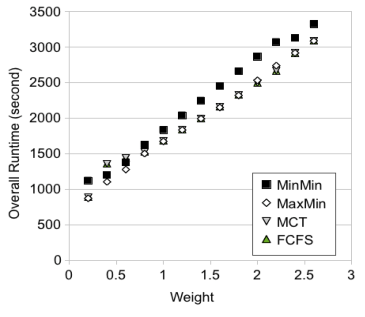
\includegraphics[width=0.6\textwidth]{figures/model/wfs_queue_delay.pdf}
%    \caption{Influence of Queue Delay. The duration of overheads are multiplied by the weights.}
%   \label{fig:model_wfs_queue_delay}
%\end{figure} 

%With the emergence of distributed heterogeneous systems, such as grids and clouds, and applications such as  large scale of workflows with  complex data dependencies, significant overheads can be incurred during workflow execution. Most of the existing DAG scheduling heuristics underestimate or even ignore the influence of workflow overheads. In such a distributed environment, a carefully crafted schedule based on deterministic and static information may fail to provide a sufficient solution. In this study, we analyze the overhead robustness of multiple static and dynamic DAG scheduling heuristics. Overhead robustness describes the influence of overheads on the workflow runtime. We investigate whether the dynamic change in workflow overheads influences the overall runtime of workflows. The reason why we are interested in this study is that in reality, system overheads are difficult to estimate or track. Existing heuristics and algorithms may have different sensitivity to the dynamic change of system overhead or the inaccurate estimation of them. Analyzing their performance in terms of the change of overheads can offer us a unique aspect of their robustness in real systems and suggest the direction of designing new heuristics or algorithms.

%\begin{figure}[h!]
%	\centering
%    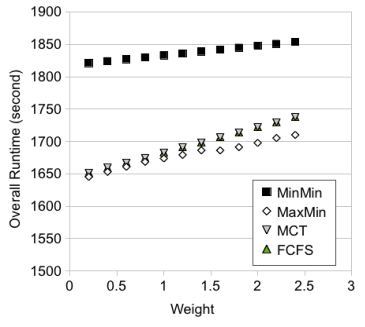
\includegraphics[width=0.6\textwidth]{figures/model/wfs_engine_delay.pdf}
%    \caption{Influence of Workflow Engine Delay}
%    \label{fig:model_wfs_engine_delay}
%\end{figure} 
%\begin{figure}[h!]
%	\centering
%    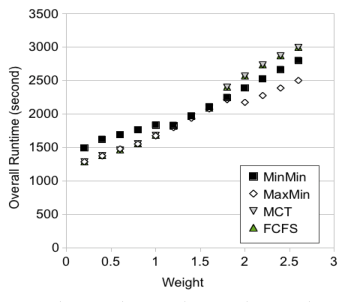
\includegraphics[width=0.6\textwidth]{figures/model/wfs_clustering_delay.pdf}
%   \caption{Influence of Clustering Delay}
%    \label{fig:model_wfs_clustering_delay}
%\end{figure} 


%In this experiment, we doubled the computation capabilities of half of the available resources so as to create an environment where heuristics and algorithms can select their allocated resources to execute workflow jobs.  We varied the duration of overheads by multiplying them with a weight that ranges from 0.2 to 2.5 in our experiment. The original workflow has the weight is 1.0. We evaluated the performance of four heuristics with the same Montage workflow used in Section VI: 
%\begin{enumerate}
%\item FCFS: First Come First Serve is the basic version of scheduling algorithm used in our simulator. It assigns each job, in the arriving order to the next available resources, regardless of the jobs’ expected completion time on that worker node. If there are multiple resources available, it randomly chooses one as the candidate. 
%\item MCT: Minimum Completion Time \cite{Braun2001} assigns each job in an arbitrary order to the available resource with the best expected completion time of that job. 
%\item MinMin: The MinMin \cite{Blythe2005} heuristic begins with a set of all free jobs and then sorts them by the order of completion time. The job with the minimum completion time is selected and assigned to the corresponding resource.  Then, the newly mapped job is submitted to the queue and the process repeats until all free jobs are scheduled. The intuition of MinMin is to create a local optimal path so as to reduce the overall runtime. 
%\item MaxMin: Similar to MinMin, but MaxMin \cite{Braun2001} picks up the job with the maximum completion time and assigns it to its best available resource. The intuition of MaxMin is to avoid penalty from long running jobs. 
%\end{enumerate}

%Experiments show that overheads have significant influence on the overall runtime and they have shown different behaviors. Fig~\ref{fig:model_wfs_queue_delay} and Fig~\ref{fig:model_wfs_engine_delay} show the influence of Queue Delay and Workflow Engine Delay respectively. Consistent with our expectation, MinMin performs worst compared to the other three methods since it assigns the best resources to small jobs while longer jobs have to wait and suffer overhead. MaxMin performs better than MCT and FCFS slightly because it tends to assign longer jobs to better resources and thereby reduces the overall runtime. Fig~\ref{fig:model_wfs_clustering_delay} shows that when the weight of Clustering Delay is lower than 1.0, MCT and FCFS perform better than MinMin. However, when the weight of Clustering Delay is larger than 2, MinMin performs better than the other two. The reason is probably because Clustering Delay only occurs to clustered jobs and in Montage these levels have better parallelism than other levels that have only non-clustered jobs. Increasing Clustering Delay thereby offers MinMin a chance to enhance its influence on the overall workflow execution. Therefore, in such an environment, the selection of heuristics is not sensitive to the estimation error of the Queue Delay or Workflow Engine Delay because the overall runtime increases at the same speed. However, the estimation error of the Clustering Delay can change the heuristics’ relative performance. 
%Only used in defense
%\subsection{Conclusion}
%In this section, we have introduced a novel workflow simulator WorkflowSim to assist researchers to evaluate their workflow optimization techniques with better accuracy and wider support than existing solutions. By comparing the results of real traces and simulation, we have validated our simulator and concluded that it is necessary to consider multiple layers of overheads and failures. In the future, we would also define more types of failures, such as the Job Submit Failure that simulates the case when a job is not successfully submitted due to a problem in workflow scheduler or a network issue between it and remote scheduler. We also plan to incorporate more workflow techniques (such as workflow partitioning) into our simulator. We will evaluate the influence of overheads in other workflow metrics besides overall runtime, for example, resource utility. 







\subsection{WorkflowSim Use cases}

WorkflowSim has attracted a wide attention in the Grid and Cloud communities and have been widely used in multiple workflow studies in literature. Below we introduce several typical use cases of WorkflowSim. 
%energy efficiency studies
\subsubsection{Energy Efficiency}


\subsubsection{Cloud Broker}
Jrad et.al. \cite{jrad2013broker} have developed a broker-based framework for running workflows in a multi-Cloud environment. They extended WorkflowSim to use the Cloud Service Broker as the scheduler instead of using an external one. In addition, a Replica Catalog keeps a list of data replicas by mapping input/output filenames to their current site locations. The data transfer is initiated by workflow tasks during their execution on the respective data-centers, whereas the Replica Catalog is managed by the Data Manager. 


\subsubsection{Balanced Task Clustering}
Recently we have used WorkflowSim to evaluate the dependency imbalance and runtime imbalance while performing task clustering in scientific workflows \cite{Chen2013b, Chen2013a}. With the support of task clustering and the modeling of data dependencies in WorkflowSim, we are able to evaluate the cause of dependency imbalance and runtime imbalance respectively and propose balanced task clustering algorithms to improve the overall performance of scientific workflows. We used traces of five widely used scientific workflows that were run on FutureGrid \cite{FutureGrid} and Amazon EC2 \cite{AmazonEC2}. 

\subsubsection{Fault Tolerant Clustering}
Many existing clustering strategies ignore or underestimate the impact of the occurrence of failures on system behavior, despite the increasing impact of failures in large-scale distributed systems. We have proposed fault tolerant clustering algorithms \cite{Chen2012} that dynamically adjusts the clustering strategy based on the current trend of failures. During the runtime, this approach estimates the failure distribution among all the resources and dynamically merges tasks into jobs of moderate size and recluster failed jobs to avoid failures. To complete this work, we relied on the generation of transient failures and reclustering techniques in WorkflowSim. 


Other than these works, WorkflowSim have been widely used to evaluate the performance of scheduling algorithms under different scenario. For example, Pooja et. al. \cite{pooja2013performance} used WorkflowSim to evaluate the cost and makespan of running scientific workflows on clouds. Prathibha et. al. \cite{prathibha2014monitoring} further evaluated the cost benefit of using task clustering in WorkflowSim. Watanabe et.al.\cite{pedro2014PowerWorkflowSim} have developed PowerWorkflowSim that extends WorkflowSim with an energy simulation API and used it to develop algorithms for energy savings in scheduling workflows in computational clouds. 


\section{Workflows Used}